%%%%%%%%%%%%%%%%%%%%%%%%
%
% $Autor: Wings $
% $Datum: 2020-07-24 09:05:07Z $
% $Pfad: GDV/Vortraege/latex - Ausarbeitung/Kapitel/Einleitung.tex $
% $Version: 4732 $
%
%%%%%%%%%%%%%%%%%%%%%%%%

\chapter{KnowledgeDiscovery in Databases (KDD) Process}

KDD plays a pivotal role in helping organizations navigate the over whelming volumes of data generated in today’s information-driven world. KDD is a structural approach to data analysis to discover and make explicit knowledge available in extensive data sets. This methodology involves a series of well-defined steps, including data selection, preprocessing, transformation and analysis, leading to the generation of actionable knowledge.

\begin{figure}
\begin{center}
		
		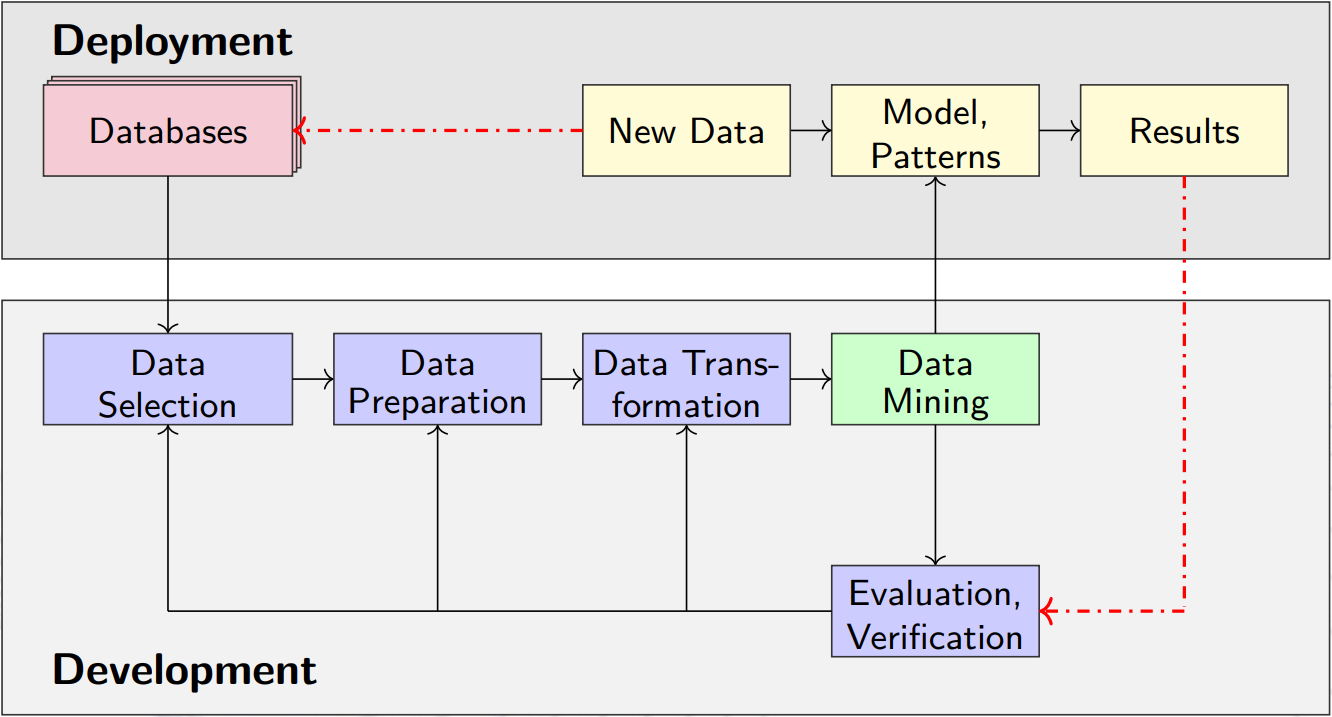
\includegraphics[width=0.4\linewidth]{images/KDD.png}
		\captionof{figure}{KDD1}
		\label{Arduino PortentaH7 Connected to a Laptop1}
\end{center}
	
\end{figure}

\begin{figure}
	\begin{center}
		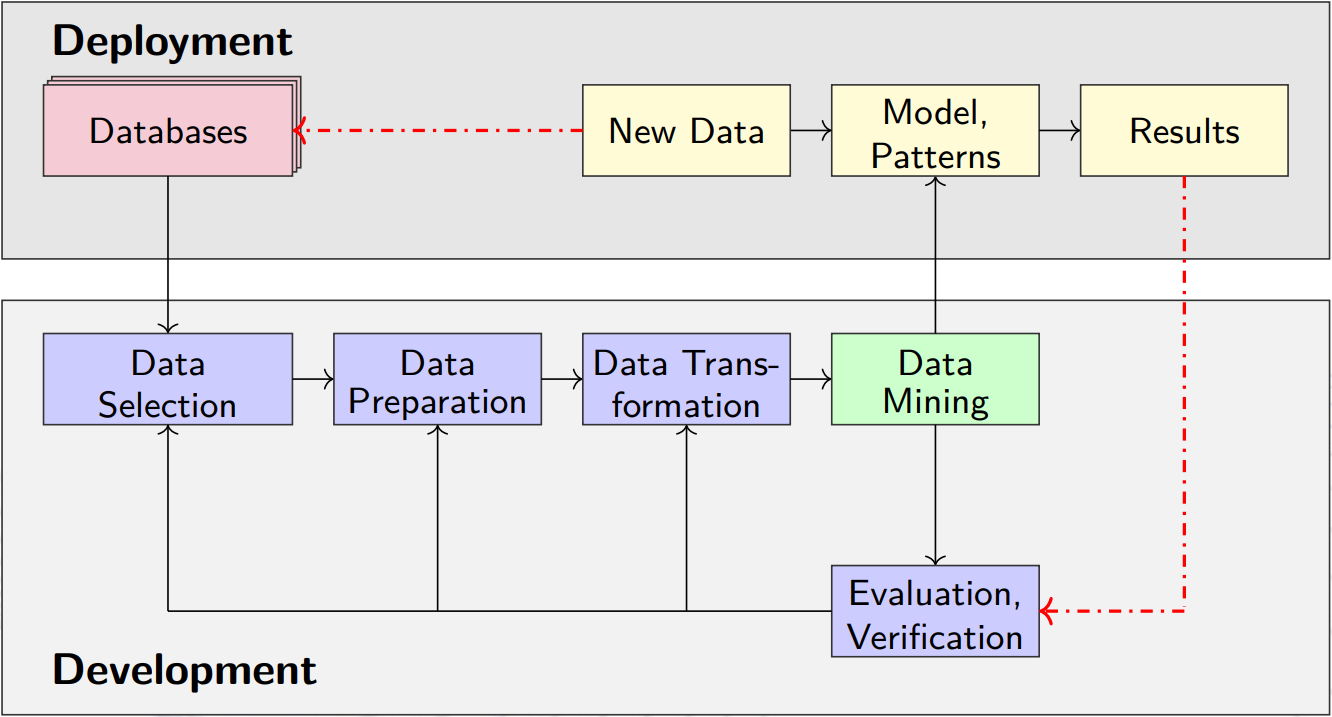
\includegraphics[width=0.7\linewidth]{Images/KDD.png}
		\caption{KDD Process2}
		\label{KDD Process2}
	\end{center}
\end{figure}

\section{Introduction}
